% interactcadsample.tex
% v1.03 - April 2017

\documentclass[]{interact}

\usepackage{epstopdf}% To incorporate .eps illustrations using PDFLaTeX, etc.
\usepackage{subfigure}% Support for small, `sub' figures and tables
%\usepackage[nolists,tablesfirst]{endfloat}% To `separate' figures and tables from text if required

\usepackage{natbib}% Citation support using natbib.sty
\bibpunct[, ]{(}{)}{;}{a}{}{,}% Citation support using natbib.sty
\renewcommand\bibfont{\fontsize{10}{12}\selectfont}% Bibliography support using natbib.sty

\theoremstyle{plain}% Theorem-like structures provided by amsthm.sty
\newtheorem{theorem}{Theorem}[section]
\newtheorem{lemma}[theorem]{Lemma}
\newtheorem{corollary}[theorem]{Corollary}
\newtheorem{proposition}[theorem]{Proposition}

\theoremstyle{definition}
\newtheorem{definition}[theorem]{Definition}
\newtheorem{example}[theorem]{Example}

\theoremstyle{remark}
\newtheorem{remark}{Remark}
\newtheorem{notation}{Notation}

% Pandoc syntax highlighting
\usepackage{color}
\usepackage{fancyvrb}
\newcommand{\VerbBar}{|}
\newcommand{\VERB}{\Verb[commandchars=\\\{\}]}
\DefineVerbatimEnvironment{Highlighting}{Verbatim}{commandchars=\\\{\}}
% Add ',fontsize=\small' for more characters per line
\usepackage{framed}
\definecolor{shadecolor}{RGB}{248,248,248}
\newenvironment{Shaded}{\begin{snugshade}}{\end{snugshade}}
\newcommand{\AlertTok}[1]{\textcolor[rgb]{0.94,0.16,0.16}{#1}}
\newcommand{\AnnotationTok}[1]{\textcolor[rgb]{0.56,0.35,0.01}{\textbf{\textit{#1}}}}
\newcommand{\AttributeTok}[1]{\textcolor[rgb]{0.13,0.29,0.53}{#1}}
\newcommand{\BaseNTok}[1]{\textcolor[rgb]{0.00,0.00,0.81}{#1}}
\newcommand{\BuiltInTok}[1]{#1}
\newcommand{\CharTok}[1]{\textcolor[rgb]{0.31,0.60,0.02}{#1}}
\newcommand{\CommentTok}[1]{\textcolor[rgb]{0.56,0.35,0.01}{\textit{#1}}}
\newcommand{\CommentVarTok}[1]{\textcolor[rgb]{0.56,0.35,0.01}{\textbf{\textit{#1}}}}
\newcommand{\ConstantTok}[1]{\textcolor[rgb]{0.56,0.35,0.01}{#1}}
\newcommand{\ControlFlowTok}[1]{\textcolor[rgb]{0.13,0.29,0.53}{\textbf{#1}}}
\newcommand{\DataTypeTok}[1]{\textcolor[rgb]{0.13,0.29,0.53}{#1}}
\newcommand{\DecValTok}[1]{\textcolor[rgb]{0.00,0.00,0.81}{#1}}
\newcommand{\DocumentationTok}[1]{\textcolor[rgb]{0.56,0.35,0.01}{\textbf{\textit{#1}}}}
\newcommand{\ErrorTok}[1]{\textcolor[rgb]{0.64,0.00,0.00}{\textbf{#1}}}
\newcommand{\ExtensionTok}[1]{#1}
\newcommand{\FloatTok}[1]{\textcolor[rgb]{0.00,0.00,0.81}{#1}}
\newcommand{\FunctionTok}[1]{\textcolor[rgb]{0.13,0.29,0.53}{\textbf{#1}}}
\newcommand{\ImportTok}[1]{#1}
\newcommand{\InformationTok}[1]{\textcolor[rgb]{0.56,0.35,0.01}{\textbf{\textit{#1}}}}
\newcommand{\KeywordTok}[1]{\textcolor[rgb]{0.13,0.29,0.53}{\textbf{#1}}}
\newcommand{\NormalTok}[1]{#1}
\newcommand{\OperatorTok}[1]{\textcolor[rgb]{0.81,0.36,0.00}{\textbf{#1}}}
\newcommand{\OtherTok}[1]{\textcolor[rgb]{0.56,0.35,0.01}{#1}}
\newcommand{\PreprocessorTok}[1]{\textcolor[rgb]{0.56,0.35,0.01}{\textit{#1}}}
\newcommand{\RegionMarkerTok}[1]{#1}
\newcommand{\SpecialCharTok}[1]{\textcolor[rgb]{0.81,0.36,0.00}{\textbf{#1}}}
\newcommand{\SpecialStringTok}[1]{\textcolor[rgb]{0.31,0.60,0.02}{#1}}
\newcommand{\StringTok}[1]{\textcolor[rgb]{0.31,0.60,0.02}{#1}}
\newcommand{\VariableTok}[1]{\textcolor[rgb]{0.00,0.00,0.00}{#1}}
\newcommand{\VerbatimStringTok}[1]{\textcolor[rgb]{0.31,0.60,0.02}{#1}}
\newcommand{\WarningTok}[1]{\textcolor[rgb]{0.56,0.35,0.01}{\textbf{\textit{#1}}}}

% tightlist command for lists without linebreak
\providecommand{\tightlist}{%
  \setlength{\itemsep}{0pt}\setlength{\parskip}{0pt}}



\usepackage{hyperref}
\usepackage[utf8]{inputenc}
\def\tightlist{}


\begin{document}


\articletype{ARTICLE TEMPLATE}

\title{Taylor \& Francis Rmarkdown template for authors (\LaTeX-based
\textsf{Interact} layout + Chicago author-date reference style)}


\author{\name{M. Galdino$^{a}$}
\affil{$^{a}$Political Science Department, Universidade de são Paulo,
Brazil.}
}

\thanks{CONTACT M.
Galdino. Email: \href{mailto:mgaldino@usp.br}{\nolinkurl{mgaldino@usp.br}}}

\maketitle

\begin{abstract}
O conceito de potências médias, apesar de sua prevalência na literatura
de Relações Internacionais (RI), enfrenta um desafio crítico de
ambiguidade conceitual que limita sua utilidade analítica. Esta pesquisa
visa abordar esse desafio propondo um novo arcabouço teórico que integra
a teoria dos jogos não cooperativa, especificamente através da adaptação
dos conceitos de estratégias complementares e substitutas. Ao fazer
isso, o projeto tem como objetivo superar as divisões teóricas
existentes e promover uma compreensão mais precisa e abrangente das
potências médias. Tradicionalmente, a RI concentrou-se na teoria do
comportamento das grandes potências, negligenciando uma teoria inclusiva
que explique o comportamento de estados de diferentes magnitudes. Este
estudo argumenta pela necessidade de uma teoria do comportamento estatal
que englobe não apenas as grandes potências, mas também as médias e
pequenas, oferecendo uma maneira empírica de diferenciar esses grupos de
países. Ao unificar as variáveis explicativas relacionadas ao poder,
comportamento e identidade dos estados, propomos um caminho para uma
validação empírica robusta, estabelecendo um programa de pesquisa
progressivo no sentido Lakatos. Além de sua contribuição teórica, este
projeto delineia um desenho de pesquisa empírica, priorizando o estudo
de cabos diplomáticos como fontes primárias. Essas fontes são
consideradas essenciais para testar as hipóteses derivadas de nossa
abordagem teórica, possibilitando uma avaliação detalhada das
estratégias adotadas pelas potências médias no cenário internacional.
Assim, o projeto não apenas promete clarificar a categorização de
potências médias, mas também fornece uma base para futuras investigações
empíricas neste campo, contribuindo significativamente para a literatura
existente e oferecendo novas ferramentas analíticas para pesquisadores e
formuladores de políticas.
\end{abstract}

\begin{keywords}
Potências Médias; Teoria dos Jogos; Estratégias Complementares;
Estratégias Substitutas; Cabos Diplomáticos;
\end{keywords}

\hypertarget{introduuxe7uxe3o}{%
\section{Introdução}\label{introduuxe7uxe3o}}

A Teoria das Potências Médias, desde seu início (cf.
\citet{chaudhuri_1969}; \citet{holbraad_71}), enfrentou problemas de
clareza analítica. A dificuldade em conceituar quem seriam as potências
médias, seja por alguma medida objetiva de poder (combinando um ou mais
indicadores) ou por seu comportamento, é reveladora dessa confusão
analítica. A despeito disso, a literatura continua a usar o conceito,
variando na forma de defini-lo e operacionalizá-lo empiricamente, assim
como nas várias tentativas de resolver os problemas conceituais.

A concepção mais tradicional de potência média é baseada na posição que
os estados ocupam no sistema internacional (por exemplo,
\citet{holbraad_84}; \citet{cooper_etal_93}; \citet{shin_12}). Assim,
países com capacidades médias ou medianas teriam um comportamento de
política externa diferente ou previsível em relação a estados com maior
ou menor capacidade. Essa diferenciação pode se dar tanto pela formação
de interesses distintos quanto pelo estilo ou estratégia de atuação na
esfera internacional (cf. \citet{cooper_11} para uma revisão da
literatura). No entanto, isso não é suficiente para operacionalizar o
conceito de maneira consistente, uma vez que não há clareza sobre qual
medida de capacidade deve ser usada (seja ela militar, econômica,
diplomática ou uma combinação dessas e de outras variáveis), a posição
relativa pode mudar dependendo da região geográfica considerada e a
inclusão de variáveis como participação em alianças, ao modificar a
medida de poder, acaba trazendo confusão analítica ao conceito
(\citet{cooper_11}). O resultado dessa confusão é a inexistência de uma
lista definida, no tempo e espaço, de quais países seriam potências
médias, o que torna inviável testar se, de fato, há um comportamento
distintivo na política externa desses países.

Em segundo lugar, há teorias focadas no comportamento desses estados. O
que seria distintivo das potências médias seria seu comportamento, tal
como a adesão ao multilateralismo, a tentativa de agir como ``bom
cidadão'', a capacidade de atuar como mediador de conflitos, etc.
(\citet{schiavon_dominguez_16}; \citet{stephen_13}; \citet{welsh_04}).

O problema óbvio dessa abordagem é a impossibilidade de explicar
comportamento com base em uma categorização do comportamento devido à
óbvia circularidade. Além disso, essa abordagem tampouco contribuiu, ao
menos, para observar um padrão de comportamento dos países
tradicionalmente concebidos como potências médias. Alguns estudos
combinam capacidades e comportamento para classificar os países, mas
isso não resolve o problema de circularidade (\citet{cooper_11}).

Por fim, mais recentemente, tem havido tentativas de conceituar potência
média a partir da identidade dos estados, em particular aqueles que se
autodefinem como potências médias (\citet{hynek_07};
\citet{gecelovsky_09}; \citet{debhal_23}).

Esse espectro conceitual sugere uma continuidade com a tradição da RI no
estudo das grandes potências. Tradicionalmente, a RI focou em uma teoria
do comportamento das grandes potências, deixando um vazio analítico
sobre o comportamento estatal além dessas. A categorização qualitativa
de ``grande potência'' ou ``superpotência'' indica que outras
categorias, como as ``potências médias'', podem ser analiticamente
úteis, embora a sua utilidade ainda seja um ponto de debate intenso.

Ante a complexidade desse cenário, parece claro que, para redescobrir a
utilidade analítica do conceito de potências médias, é necessário um
trabalho teórico e empírico de grandes proporções. Do lado teórico,
parece-nos claro que qualquer que seja o marcador ou marcadores que
distingam potências médias, essas variáveis precisam estar relacionadas
também ao comportamento dos estados de outros tamanhos. Isso sugere que
a pesquisa empírica nessa área precisa ser comparativa e incluir não
apenas as pretensas potências médias, mas também os países que estariam
em outras categorias.

O presente trabalho, portanto, parte dessa ambição como horizonte de
pesquisa. Por outro lado, este é um projeto laborioso e que exigirá
esforço colaborativo para ser empreendido. Assim, o que apresentamos a
seguir é nossa estratégia para um primeiro passo nessa direção, sem a
pretensão de delinear o caminho todo a ser percorrido. Além de ser mais
realista, parece-nos mais efetivo, na medida em que facilita a correção
de rotas que o trabalho de pesquisa e as descobertas não antecipadas
demandam.

No nível teórico, o presente trabalho propõe uma solução ancorada em uma
adaptação dos conceitos de estratégias complementares e substitutas da
teoria dos jogos não cooperativa. Esta abordagem promete superar a
ambiguidade conceitual em torno das potências médias, unificando os
comportamentos dos estados numa única teoria que explique a
diferenciação entre os três grupos de países - grandes, médias e
pequenas potências. Argumentamos que tal teoria, ao enfatizar a
centralidade das relações entre estratégias dos países em diferentes
arenas de conflito (se complementares ou substitutas), abre caminho para
uma nova agenda de pesquisa empírica.

No nível teórico, o presente trabalho propõe uma solução ancorada em uma
adaptação dos conceitos de estratégias complementares e substitutas da
teoria dos jogos não cooperativa. Esta abordagem promete superar a
ambiguidade conceitual em torno das potências médias, unificando os
comportamentos dos estados numa única teoria que explique a
diferenciação entre os três grupos de países - grandes, médias e
pequenas potências. Argumentamos que tal teoria, ao enfatizar a
centralidade das relações entre estratégias dos países em diferentes
arenas de conflito (se complementares ou substitutas), abre caminho para
uma nova agenda de pesquisa empírica.

Do ponto de vista empírico, pretendemos construir uma base de dados de
cabos diplomáticos de países em perspectiva comparada, consistindo de
países dos mais variados tamanhos. A recente proliferação das leis de
acesso à informação e iniciativas de dados abertos mundo afora
(\citet{zuffova_20}) possibilita que, finalmente, tal tarefa possa ser
empreendida com boa chance de sucesso.

Este estudo busca, portanto, consolidar a teoria de potências médias
como um programa de pesquisa progressivo, no sentido proposto por
Lakatos, mediante a conexão de variáveis explicativas - sejam elas
relativas a poder, comportamento ou identidade - com hipóteses causais
testáveis empiricamente.

A abordagem proposta oferece um caminho promissor para a superação dos
desafios conceituais e metodológicos que têm caracterizado o estudo das
potências médias até o momento. Por fim, pretendemos ilustrar essa
perspectiva com um estudo de caso focado no Brasil e EUA, estudando os
cabos diplomáticos disponíveis para ambos os países.

Nas próximas seções, desenvolvemos um pouco mais o arcabouço teórico,
para ilustrar o tipo de teorização que será realizada, e, em seguida,
apresentamos como se dará a pesquisa empírica no estudo de caso que
pretendemos realizar.

\hypertarget{modelo-teuxf3rico}{%
\subsection{Modelo Teórico}\label{modelo-teuxf3rico}}

Em um artigo seminal sobre a aplicação da teoria dos jogos à economia,
\citet{bulow_etal_85} introduziu a ideia de jogos com estratégias
complementares ou substitutas. Considerando as estratégias como
variáveis contínuas (e.g., nível de investimento), estratégias são ditas
complementares se o aumento no nível de uma estratégia por um agente
torna ótimo para outro agente aumentar o nível de sua própria
estratégia. Matematicamente, isso ocorre quando a derivada parcial
cruzada do payoff de um agente, em relação à sua estratégia e à do outro
jogador, é positiva. Em contraste, estratégias são substitutas quando o
aumento na estratégia de um agente leva o outro a reduzir a sua,
evidenciado por uma derivada parcial cruzada negativa.

O exemplo arquetípico apresentado por \citet{bulow_etal_1985} envolve
dois mercados, \(1\) e \(2\), com demandas independentes onde a empresa
\(A\) monopoliza o primeiro mercado e compete com a empresa \(B\) no
segundo. Como os produtos de \(A\) e \(B\) no mercado \(2\) são
substitutos, o modelo de equilíbrio de Cournot demonstra que um
comportamento mais agressivo de \(A\) no mercado \(1\) induz a empresa
\(B\) a ser menos agressiva no mercado \(2\), evidenciando a
substitutividade das estratégias.

Esse modelo tem implicações significativas ao ser transportado para o
contexto das Relações Internacionais, sugerindo que o ganho de um estado
\(A\) derivado de uma mudança em um jogo \(1\) é afetado pela sua
posição em um jogo \(B\), seja como grande potência (monopolista),
potência média (oligopolista) ou pequena potência (competidor puro).

A aplicação deste arcabouço às Relações Internacionais permite discutir
como grandes potências distinguem-se das potências médias pela
capacidade de alterar os termos do jogo \(1\), induzindo comportamentos
específicos nos países envolvidos. Da mesma forma, potências médias
podem adotar comportamentos de coalizões empreendedoras de norma
(\citet{ravenhill_2018}), alterando exogenamente os custos para países
em um jogo A, para induzir mudanças de comportamento em um jogo B.

Para ilustrar o potencial analítico desse arcabouço, propomos um esboço
informal de dois jogos distintos, demonstrando como a presença de
estratégias complementares ou substitutas explica certos comportamentos
e auxilia na categorização dos tamanhos das potências.

Diferentemente da literatura existente, nossa abordagem torna a
categorização de potência média dependente da estrutura da conectividade
dos jogos. Assim, podemos clarificar a confusão conceitual presente na
definição de potências médias na literatura, utilizando medidas de
capacidade que influenciam a estrutura (complementar ou substituta) das
estratégias, enquanto incorporamos variáveis contextuais (como a
participação em alianças) e a identidade dos atores, na medida em que
afetam suas preferências. Além disso, ao propor um mecanismo específico,
podemos testar empiricamente as hipóteses derivadas dos modelos sem
incorrer em circularidade argumentativa.

\hypertarget{modelos-de-estratuxe9gias-complementares-e-substitutas}{%
\subsection{Modelos de Estratégias Complementares e
Substitutas}\label{modelos-de-estratuxe9gias-complementares-e-substitutas}}

Considere um jogo entre dois estados, \(A\) e \(B\), disputando um
território de valor \(X = [0,1]\), conforme proposto por Fearon (1995).
O estado \(A\) prefere um resultado próximo de \(1\), enquanto \(B\)
favorece um resultado próximo de \(0\). Na negociação diplomática para o
conflito, o resultado será denotado por \(x \in X\), com as utilidades
\(u_A(x)\) para \(A\) e \(u_B(1-x)\) para \(B\). Cada estado possui uma
utilidade esperada da guerra dada por: \(p_a u(1) + (1-p)u(0) - c_a\)
para \(A\) e uma fórmula similar para \(B\), com custo \(c_b\). Segundo
o modelo de barganha de Rubinstein, com horizonte infinito onde as
partes fazem ofertas alternadas e excluindo temporariamente a opção de
guerra, o equilíbrio de Nash perfeito em sub-jogo (sem a opção de
guerra) seria dado por \((x, 1-x)\), onde
\(x = \frac{1 -\delta_A}{1 - \delta_A \delta_B}\). A opção da guerra, no
entanto, restringe os valores de \((x, 1-x)\) que são preferíveis à
guerra, com \(x > \mathbb{E}[u^g_A]\) e \(1 - x > \mathbb{E}[u^g_B]\)
para que a opção diplomática seja estritamente preferível para ambos.

A utilidade de estratégias complementares ou substitutas neste contexto
torna-se evidente ao considerar diferentes cenários envolvendo grandes
potências, potências médias e países pequenos. Por exemplo, em um
cenário onde o estado \(A\) é uma grande potência, a decisão sobre a
alocação de recursos militares próximo à fronteira em conflito pode
aumentar a sua probabilidade de vitória, influenciando assim as
estratégias de negociação.

Em contraste, em um conflito sobre a expropriação de uma empresa
estrangeira, como um setor de extração de petróleo, a presença de um
aliado do país \(B\) pode compelir o país \(A\) a ceder mais na
negociação para não prejudicar a aliança com o país \(C\). Isso ilustra
como estratégias em um jogo podem influenciar os resultados de outro.

\hypertarget{literatura-relacionada}{%
\subsection{Literatura Relacionada}\label{literatura-relacionada}}

A interconexão entre jogos distintos e suas consequências nas decisões
dos jogadores é um conceito que já foi explorado no campo das Relações
Internacionais, particularmente na teoria de jogos de dois níveis de
Putnam (1988) e suas subsequentes ampliações e aplicações. Entretanto,
nosso framework se distingue ao aplicar-se a qualquer conexão entre
jogos distintos, proporcionando insights únicos sobre a dinâmica de
estratégias complementares e substitutas.

Outra abordagem relacionada é a de ``issue linkages'' (Tollison \&
Willett, 1979), que embora compartilhe algumas semelhanças com nosso
framework, difere na medida em que foca na construção de acordos
multidimensionais que geram benefícios mútuos, sem necessariamente
antecipar as complementaridades ou substitutibilidades estratégicas.

Note that any \texttt{footnote}s to the main text will automatically be
assigned the superscript symbols 1, 2, 3, etc. by the class
file.\footnote{If preferred, the \texttt{endnotes} package may be used
  to set the notes at the end of your text, before the bibliography. The
  symbols will be changed to match the style of the journal if necessary
  by the typesetter.}

\hypertarget{embedding-r-code}{%
\section{Embedding R code}\label{embedding-r-code}}

\hypertarget{code-chunks}{%
\subsection{Code chunks}\label{code-chunks}}

\begin{Shaded}
\begin{Highlighting}[]
\FunctionTok{summary}\NormalTok{(cars)}
\end{Highlighting}
\end{Shaded}

\begin{verbatim}
##      speed           dist       
##  Min.   : 4.0   Min.   :  2.00  
##  1st Qu.:12.0   1st Qu.: 26.00  
##  Median :15.0   Median : 36.00  
##  Mean   :15.4   Mean   : 42.98  
##  3rd Qu.:19.0   3rd Qu.: 56.00  
##  Max.   :25.0   Max.   :120.00
\end{verbatim}

\hypertarget{including-plots}{%
\subsection{Including Plots}\label{including-plots}}

You can also embed plots, for example:

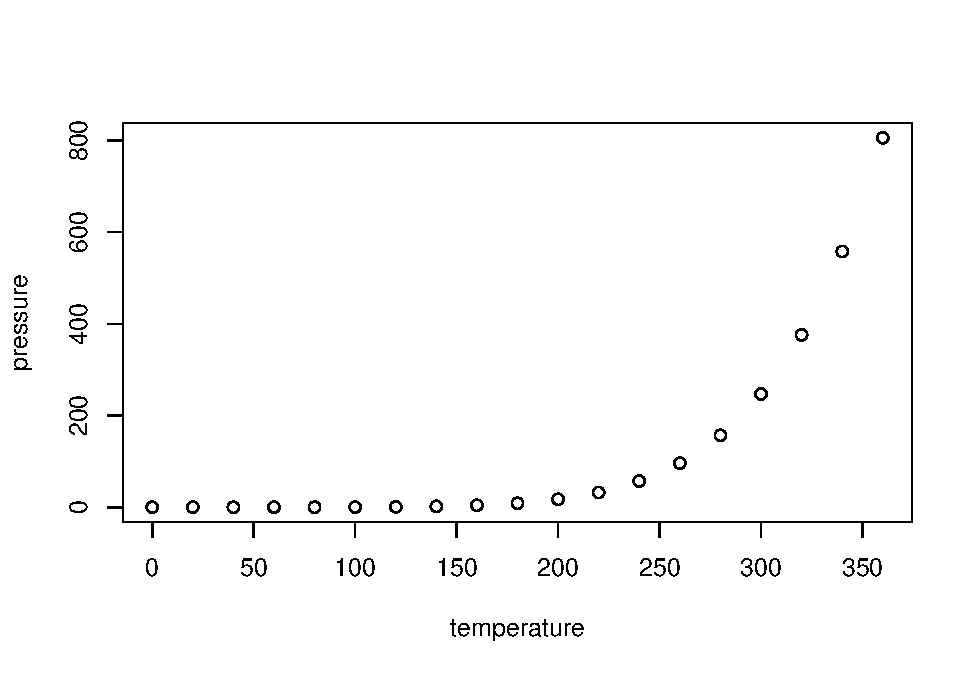
\includegraphics[width=0.8\linewidth]{research_project_files/figure-latex/pressure-1}

Note that the \texttt{echo\ =\ FALSE} parameter was added to the code
chunk to prevent printing of the R code that generated the plot.

\hypertarget{some-guidelines-for-using-the-standard-features-of}{%
\section{\texorpdfstring{Some guidelines for using the standard features
of
\LaTeX}{Some guidelines for using the standard features of }}\label{some-guidelines-for-using-the-standard-features-of}}

\hypertarget{sections}{%
\subsection{Sections}\label{sections}}

The \textsf{Interact} layout style allows for five levels of section
heading, all of which are provided in the \texttt{interact} class file
using the standard \LaTeX~commands \texttt{\textbackslash{}section},
\texttt{\textbackslash{}subsection},
\texttt{\textbackslash{}subsubsection},
\texttt{\textbackslash{}paragraph} and
\texttt{\textbackslash{}subparagraph}. Numbering will be automatically
generated for all these headings by default.

\hypertarget{lists}{%
\subsection{Lists}\label{lists}}

Numbered lists are produced using the \texttt{enumerate} environment,
which will number each list item with arabic numerals by default. For
example,

\begin{enumerate}
\def\labelenumi{\arabic{enumi}.}
\tightlist
\item
  first item
\item
  second item
\item
  third item
\end{enumerate}

Alternative numbering styles can be achieved by inserting an optional
argument in square brackets to each \texttt{item},
e.g.~\texttt{\textbackslash{}item{[}(i){]}\ first\ item}, to create a
list numbered with roman numerals at level one.

Bulleted lists are produced using the \texttt{itemize} environment. For
example,

\begin{itemize}
\tightlist
\item
  First bulleted item
\item
  Second bulleted item
\item
  Third bulleted item
\end{itemize}

\hypertarget{figures}{%
\subsection{Figures}\label{figures}}

\begin{Shaded}
\begin{Highlighting}[]
\FunctionTok{plot}\NormalTok{(pressure)}
\end{Highlighting}
\end{Shaded}

The \texttt{interact} class file will deal with positioning your figures
in the same way as standard \LaTeX. It should not normally be necessary
to use the optional \texttt{{[}htb{]}} location specifiers of the
\texttt{figure} environment in your manuscript; you may, however, find
the \texttt{{[}p{]}} placement option or the \texttt{endfloat} package
useful if a journal insists on the need to separate figures from the
text.

Figure captions appear below the figures themselves, therefore the
\texttt{\textbackslash{}caption} command should appear after the body of
the figure. For example, Figure\textasciitilde{}\ref{sample-figure} with
caption and sub-captions is produced using the following commands:

\begin{verbatim}
\begin{figure}
\centering
\subfigure[An example of an individual figure sub-caption.]{%
\resizebox*{5cm}{!}{\includegraphics{path/to/fig}}}\hspace{5pt}
\subfigure[A slightly shorter sub-caption.]{%
\resizebox*{5cm}{!}{\includegraphics{path/to/fig}}}
\caption{Example of a two-part figure with individual sub-captions
 showing that captions are flush left and justified if greater
 than one line of text.} \label{sample-figure}
\end{figure}
\end{verbatim}

\begin{figure}
\centering
\subfigure[An example of an individual figure sub-caption.]{%
\resizebox*{5cm}{!}{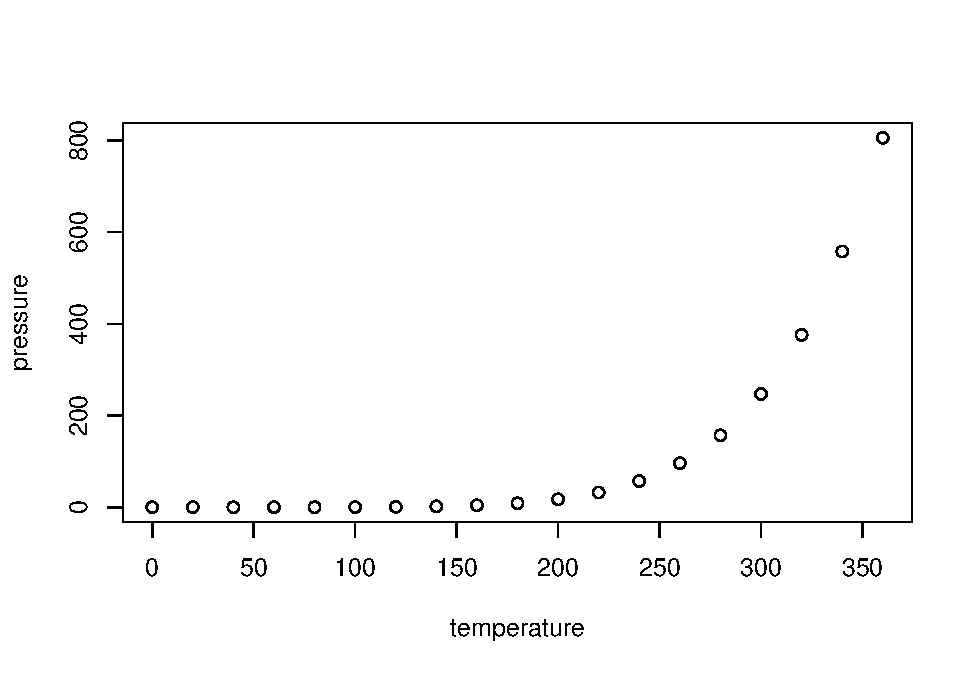
\includegraphics{research_project_files/figure-latex/pressure-plot-1.pdf}}}\hspace{5pt}
\subfigure[A slightly shorter sub-caption.]{%
\resizebox*{5cm}{!}{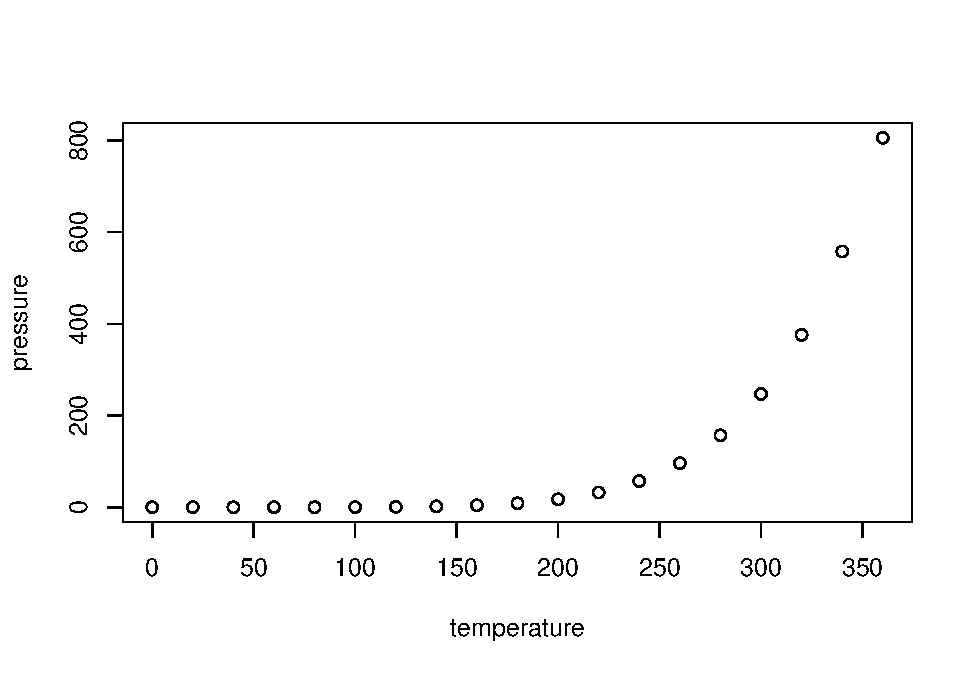
\includegraphics{research_project_files/figure-latex/pressure-plot-1.pdf}}}
\caption{Example of a two-part figure with individual sub-captions
 showing that captions are flush left and justified if greater
 than one line of text.} \label{sample-figure}
\end{figure}

To ensure that figures are correctly numbered automatically, the
\texttt{\textbackslash{}label} command should be included just after the
\texttt{\textbackslash{}caption} command, or in its argument.

The \texttt{\textbackslash{}subfigure} command requires
\texttt{subfigure.sty}, which is called in the preamble of the
\texttt{interacttfssample.tex} file (to allow your choice of an
alternative package if preferred) and included in the \textsf{Interact}
\LaTeX~bundle for convenience. Please supply any additional figure
macros used with your article in the preamble of your .tex file.

The source files of any figures will be required when the final, revised
version of a manuscript is submitted. Authors should ensure that these
are suitable (in terms of lettering size, etc.) for the reductions they
envisage.

The \texttt{epstopdf} package can be used to incorporate encapsulated
PostScript (.eps) illustrations when using PDF\LaTeX, etc. Please
provide the original .eps source files rather than the generated PDF
images of those illustrations for production purposes.

\hypertarget{tables}{%
\subsection{Tables}\label{tables}}

The \texttt{interact} class file will deal with positioning your tables
in the same way as standard \LaTeX. It should not normally be necessary
to use the optional \texttt{{[}htb{]}} location specifiers of the
\texttt{table} environment in your manuscript; you may, however, find
the \texttt{{[}p{]}} placement option or the \texttt{endfloat} package
useful if a journal insists on the need to separate tables from the
text.

The \texttt{tabular} environment can be used as shown to create tables
with single horizontal rules at the head, foot and elsewhere as
appropriate. The captions appear above the tables in the
\textsf{Interact} style, therefore the \texttt{\textbackslash{}tbl}
command should be used before the body of the table. For example,
Table\textasciitilde{}\ref{sample-table} is produced using the following
commands:

\begin{table}
\tbl{Example of a table showing that its caption is as wide as
 the table itself and justified.}
{\begin{tabular}{lcccccc} \toprule
 & \multicolumn{2}{l}{Type} \\ \cmidrule{2-7}
 Class & One & Two & Three & Four & Five & Six \\ \midrule
 Alpha\textsuperscript{a} & A1 & A2 & A3 & A4 & A5 & A6 \\
 Beta & B2 & B2 & B3 & B4 & B5 & B6 \\
 Gamma & C2 & C2 & C3 & C4 & C5 & C6 \\ \bottomrule
\end{tabular}}
\tabnote{\textsuperscript{a}This footnote shows how to include
 footnotes to a table if required.}
\label{sample-table}
\end{table}

\begin{verbatim}
\begin{table}
\tbl{Example of a table showing that its caption is as wide as
 the table itself and justified.}
{\begin{tabular}{lcccccc} \toprule
 & \multicolumn{2}{l}{Type} \\ \cmidrule{2-7}
 Class & One & Two & Three & Four & Five & Six \\ \midrule
 Alpha\textsuperscript{a} & A1 & A2 & A3 & A4 & A5 & A6 \\
 Beta & B2 & B2 & B3 & B4 & B5 & B6 \\
 Gamma & C2 & C2 & C3 & C4 & C5 & C6 \\ \bottomrule
\end{tabular}}
\tabnote{\textsuperscript{a}This footnote shows how to include
 footnotes to a table if required.}
\label{sample-table}
\end{table}
\end{verbatim}

To ensure that tables are correctly numbered automatically, the
\texttt{\textbackslash{}label} command should be included just before
\texttt{\textbackslash{}end\{table\}}.

The \texttt{\textbackslash{}toprule}, \texttt{\textbackslash{}midrule},
\texttt{\textbackslash{}bottomrule} and
\texttt{\textbackslash{}cmidrule} commands are those used by
\texttt{booktabs.sty}, which is called by the \texttt{interact} class
file and included in the \textsf{Interact} \LaTeX~bundle for
convenience. Tables produced using the standard commands of the
\texttt{tabular} environment are also compatible with the
\texttt{interact} class file.

\hypertarget{landscape-pages}{%
\subsection{Landscape pages}\label{landscape-pages}}

If a figure or table is too wide to fit the page it will need to be
rotated, along with its caption, through 90\(^{\circ}\) anticlockwise.
Landscape figures and tables can be produced using the \texttt{rotating}
package, which is called by the \texttt{interact} class file. The
following commands (for example) can be used to produce such pages.

\begin{verbatim}
\setcounter{figure}{1}
\begin{sidewaysfigure}
\centerline{\epsfbox{figname.eps}}
\caption{Example landscape figure caption.}
\label{landfig}
\end{sidewaysfigure}
\end{verbatim}

\begin{verbatim}
\setcounter{table}{1}
\begin{sidewaystable}
 \tbl{Example landscape table caption.}
  {\begin{tabular}{@{}llllcll}
    .
    .
    .
  \end{tabular}}\label{landtab}
\end{sidewaystable}
\end{verbatim}

Before any such float environment, use the
\texttt{\textbackslash{}setcounter} command as above to fix the
numbering of the caption (the value of the counter being the number
given to the preceding figure or table). Subsequent captions will then
be automatically renumbered accordingly. The
\texttt{\textbackslash{}epsfbox} command requires \texttt{epsfig.sty},
which is called by the \texttt{interact} class file and is also included
in the \textsf{Interact} \LaTeX~bundle for convenience.

Please note that if the \texttt{endfloat} package is used, one or both
of the commands

\begin{verbatim}
\DeclareDelayedFloatFlavor{sidewaysfigure}{figure}
\DeclareDelayedFloatFlavor{sidewaystable}{table}
\end{verbatim}

will need to be included in the preamble of your .tex file, after the
\texttt{endfloat} package is loaded, in order to process any landscape
figures and/or tables correctly.

\hypertarget{theorem-like-structures}{%
\subsection{Theorem-like structures}\label{theorem-like-structures}}

A predefined \texttt{proof} environment is provided by the
\texttt{amsthm} package (which is called by the \texttt{interact} class
file), as follows:

\begin{proof}
More recent algorithms for solving the semidefinite programming relaxation are particularly efficient, because they explore the structure of the MAX-CUT problem.
\end{proof}

\noindent This was produced by simply typing:

\begin{verbatim}
\begin{proof}
More recent algorithms for solving the semidefinite programming
relaxation are particularly efficient, because they explore the
structure of the MAX-CUT problem.
\end{proof}
\end{verbatim}

Other theorem-like environments (theorem, definition, remark, etc.) need
to be defined as required, e.g.~using
\texttt{\textbackslash{}newtheorem\{theorem\}\{Theorem\}} in the
preamble of your .tex file (see the preamble of
\texttt{interactcadsample.tex} for more examples). You can define the
numbering scheme for these structures however suits your article best.
Please note that the format of the text in these environments may be
changed if necessary to match the style of individual journals by the
typesetter during preparation of the proofs.

\hypertarget{mathematics}{%
\subsection{Mathematics}\label{mathematics}}

\hypertarget{displayed-mathematics}{%
\subsubsection{Displayed mathematics}\label{displayed-mathematics}}

The \texttt{interact} class file will set displayed mathematical
formulas centred on the page without equation numbers if you use the
\texttt{displaymath} environment or the equivalent
\texttt{\textbackslash{}{[}...\textbackslash{}{]}} construction. For
example, the equation \[
 \hat{\theta}_{w_i} = \hat{\theta}(s(t,\mathcal{U}_{w_i}))
\] was typeset using the commands

\begin{verbatim}
\[
 \hat{\theta}_{w_i} = \hat{\theta}(s(t,\mathcal{U}_{w_i}))
\]
\end{verbatim}

For those of your equations that you wish to be automatically numbered
sequentially throughout the text for future reference, use the
\texttt{equation} environment, e.g. \begin{equation}
 \hat{\theta}_{w_i} = \hat{\theta}(s(t,\mathcal{U}_{w_i}))
\end{equation} was typeset using the commands

\begin{verbatim}
\begin{equation}
 \hat{\theta}_{w_i} = \hat{\theta}(s(t,\mathcal{U}_{w_i}))
\end{equation}
\end{verbatim}

Part numbers for sets of equations may be generated using the
\texttt{subequations} environment, e.g.
\begin{subequations} \label{subeqnexample}
\begin{equation}
     \varepsilon \rho w_{tt}(s,t) = N[w_{s}(s,t),w_{st}(s,t)]_{s},
     \label{subeqnparta}
\end{equation}
\begin{equation}
     w_{tt}(1,t)+N[w_{s}(1,t),w_{st}(1,t)] = 0,
     \label{subeqnpartb}
\end{equation}
\end{subequations} which was typeset using the commands

\begin{verbatim}
\begin{subequations} \label{subeqnexample}
\begin{equation}
     \varepsilon \rho w_{tt}(s,t) = N[w_{s}(s,t),w_{st}(s,t)]_{s},
     \label{subeqnparta}
\end{equation}
\begin{equation}
     w_{tt}(1,t)+N[w_{s}(1,t),w_{st}(1,t)] = 0,   \label{subeqnpartb}
\end{equation}
\end{subequations}
\end{verbatim}

Displayed mathematics should be given end-of-line punctuation
appropriate to the running text sentence of which it forms a part, if
required.

\hypertarget{math-fonts}{%
\subsubsection{Math fonts}\label{math-fonts}}

\hypertarget{superscripts-and-subscripts}{%
\paragraph{Superscripts and
subscripts}\label{superscripts-and-subscripts}}

Superscripts and subscripts will automatically come out in the correct
size in a math environment (i.e.~enclosed within
\texttt{\textbackslash{}(...\textbackslash{})} or \texttt{\$...\$}
commands in running text, or within
\texttt{\textbackslash{}{[}...\textbackslash{}{]}} or the
\texttt{equation} environment for displayed equations). Sub/superscripts
that are physical variables should be italic, whereas those that are
labels should be roman (e.g.~\(C_p\), \(T_\mathrm{eff}\)). If the
subscripts or superscripts need to be other than italic, they must be
coded individually.

\hypertarget{upright-greek-characters-and-the-upright-partial-derivative-sign}{%
\paragraph{Upright Greek characters and the upright partial derivative
sign}\label{upright-greek-characters-and-the-upright-partial-derivative-sign}}

Upright lowercase Greek characters can be obtained by inserting the
letter \texttt{u} in the control code for the character,
e.g.~\texttt{\textbackslash{}umu} and \texttt{\textbackslash{}upi}
produce \(\umu\) (used, for example, in the symbol for the unit microns
-- \(\umu\mathrm{m}\)) and \(\upi\) (the ratio of the circumference of a
circle to its diameter). Similarly, the control code for the upright
partial derivative \(\upartial\) is \texttt{\textbackslash{}upartial}.
Bold lowercase as well as uppercase Greek characters can be obtained by
\texttt{\{\textbackslash{}bm\ \textbackslash{}gamma\}}, for example,
which gives \({\bm \gamma}\), and
\texttt{\{\textbackslash{}bm\ \textbackslash{}Gamma\}}, which gives
\({\bm \Gamma}\).

\bibliographystyle{tfcad}
\bibliography{Middle-Powers-bib.bib}


\input{"appendix.tex"}



\end{document}
